\subsection{Booster neutrino beam, BNB}

A Booster Neutrino Beam (BNB) of muon neutrinos is formed by firing protons, taken from an accelerator with $\sim$8 GeV kintetic energy, at a beryllium target which produces a hadronic beam consisting mainly of pions. The pions in this beam are then focussed and polarised before they decay, mostly to muon neutrinos, which propagate into the TPC where they interact with the target material. The beam's high muon neutrino excess occurs because the dominant decay channel of pions is ~(\ref{eq:piDecay}) \cite{sbn},

\begin{equation}\label{eq:piDecay}
    \pi ^{ + } \longrightarrow \mu ^{ + } + \nu _{ \mu } 
\end{equation}
    
    and the branching ratio of pions decaying to electrons over muons on the order of $\sim 10 ^{ -4 }$ due to the relation given in equation~(\ref{eq:BR}) \cite{BR}.

\begin{equation}\label{eq:BR}
    R_{ \pi } = \left( \dfrac{ m_{ e } }{ m_{ \mu } } \right) ^{2} \left( \dfrac{ m_{ \pi }^{ 2 } - m_{ e } ^{ 2 } }{ m_{ \pi } ^{ 2 } - m_{ \mu } ^{ 2 } } \right) ^{ 2 } \sim 10^{-4}
\end{equation}

The beam fires neutrinos directly into the time projection chamber (TPC) of an experiment at such velocities that it can always be assumed that the particles entered the TPC from one direction and, before iteracting, were forward-going. This technicality gives an immediate criteria for the removal of backgrounds, such as cosmogenic neutrinos, which would enter the TPC from all directions \cite{sbn}.

    
\subsection{Liquid argon time projection chambers, LArTPC}     
    
    In current and future neutrino experiments such as DUNE and the short baseline neutrino (SBN) program (SBND, MicroBooNE and ICARUS), liquid argon is the target material of the detector. Argon in this form is used due to its stability and purity as a noble gas, its high denisty and its low cost. These properties lead to resolution capabilities on the order of the Bubble Chamber experiments, which allows for high certainty in distinguishing between interactions and ultimately optimises the resolving power of the experiment \cite{larRes}. An example event display in liquid argon from the MicroBooNE experiment is given in Figure~\ref{fig:ev_disp} \cite{evDisp}.

    % Event display
    \begin{figure}[h!]
        \center
        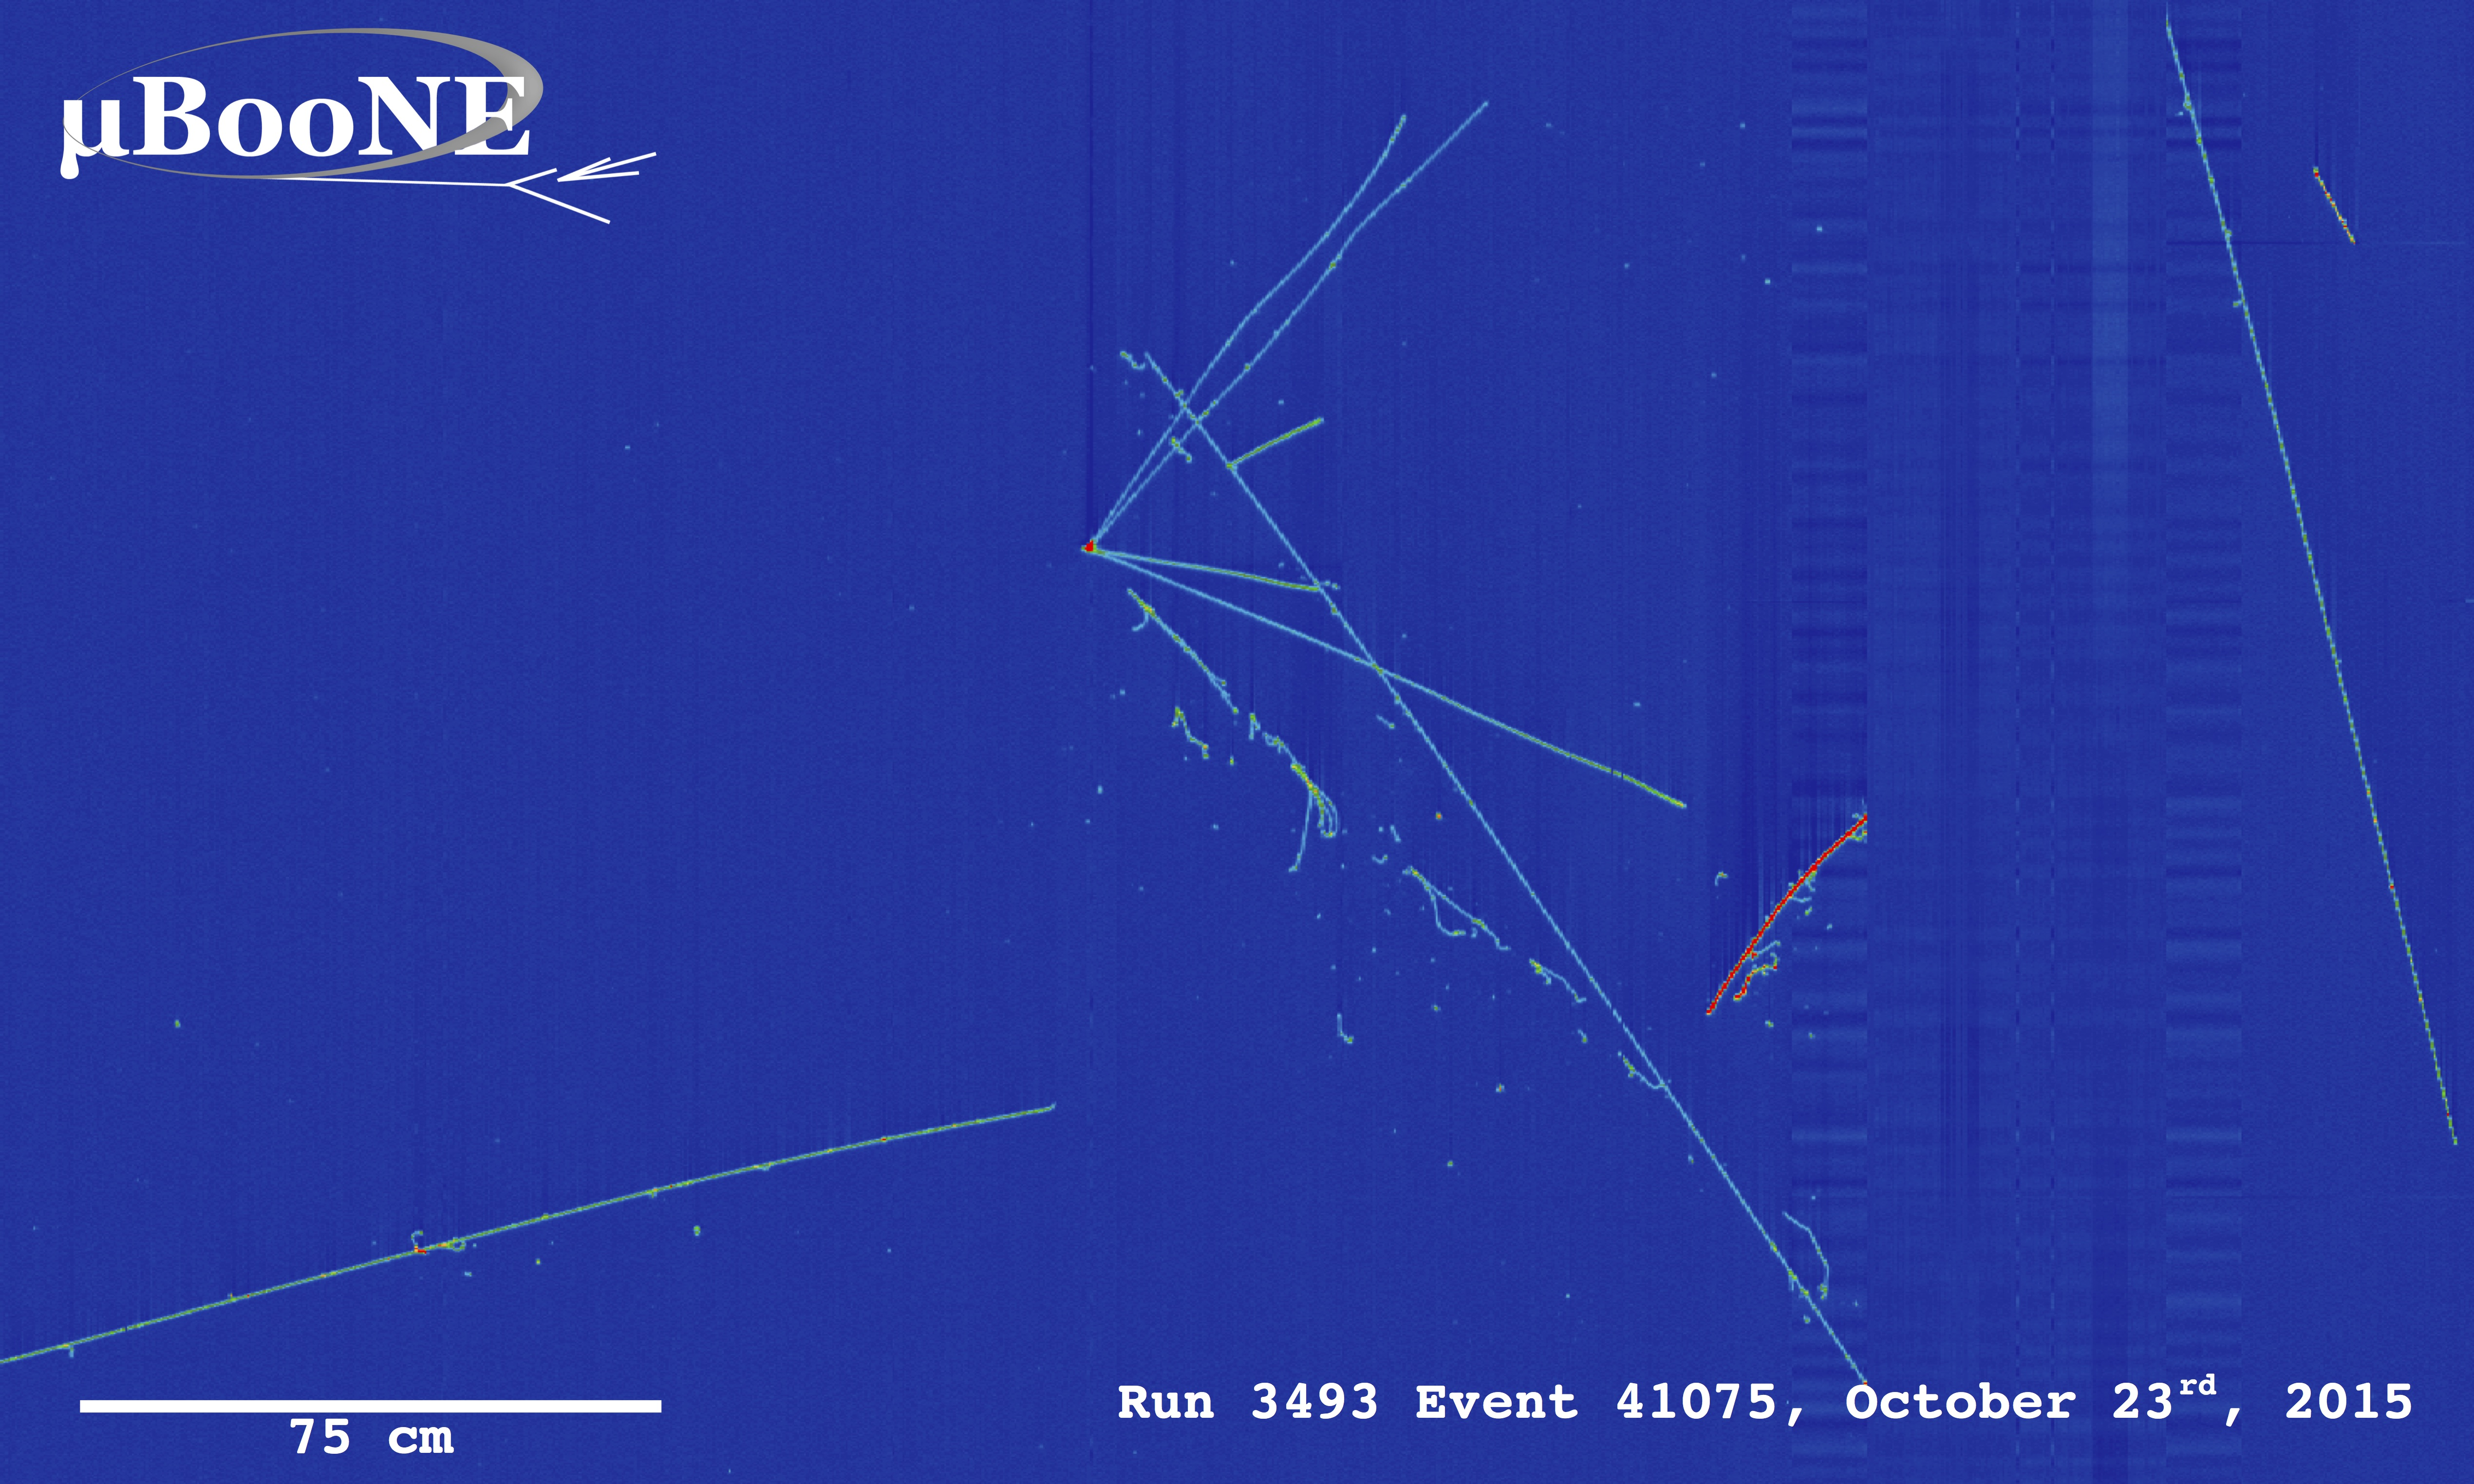
\includegraphics[width=.8\textwidth]{images/uboone_ev.png}
        \caption{An example event display from the MicroBooNE detector, one of the first to be seen in a liquid argon TPC. The resolving power is high enough for the tracks and showers to be clearly distinguished, along with the interaction vertex of the event \cite{evDisp}.}
        \label{fig:ev_disp}
    \end{figure}

Once the neutrino has entered the TPC it interacts with an argon atom to produce final state particles in the detector. These particles may then decay, be asorbed or interact with the argon in the TPC. Ionazation electrons and photons are also produced through these interactions.

A general purpose LArTPC diagram is given in Figure~\ref{fig:lartpc}. A brief description of its functionality is as follows~\cite{lartpc}: 

\newpage

\begin{itemize} 
    
    \item A potential difference is induced between the cathode and anode planes
    
    \begin{itemize}
        \item Electric field is induced by the potential difference
        \item Ionization eletrons are caused to drift towards the three planes of wires on the opposite, anode side of the TPC
    \end{itemize}

    \item Electron hits on the wires are converted to a current read out 
    
    \begin{itemize}
        \item Timing and spatial information deduced about the event
    \end{itemize}
    
    \item Induction wire planes, U \& V are situated at 60$^{\circ}$ to the vertical collection plane, Y
    
    \begin{itemize}
        \item Full 3 dimensional read out is possible
        \item Spatial information gives the y \& z co-ordinates 
        \item Timing information determines the x co-ordinate
    \end{itemize}

    \item Photons cascade into showers and reach the wall of PMTs residing behind the wire planes

    \begin{itemize}
        \item Prompt scintillation light hits the PMTs
        \item Provides additional information about the x co-ordinate of the event
    \end{itemize}

\end{itemize}

    %LArTPC
    \begin{figure}[h!]
        \center
        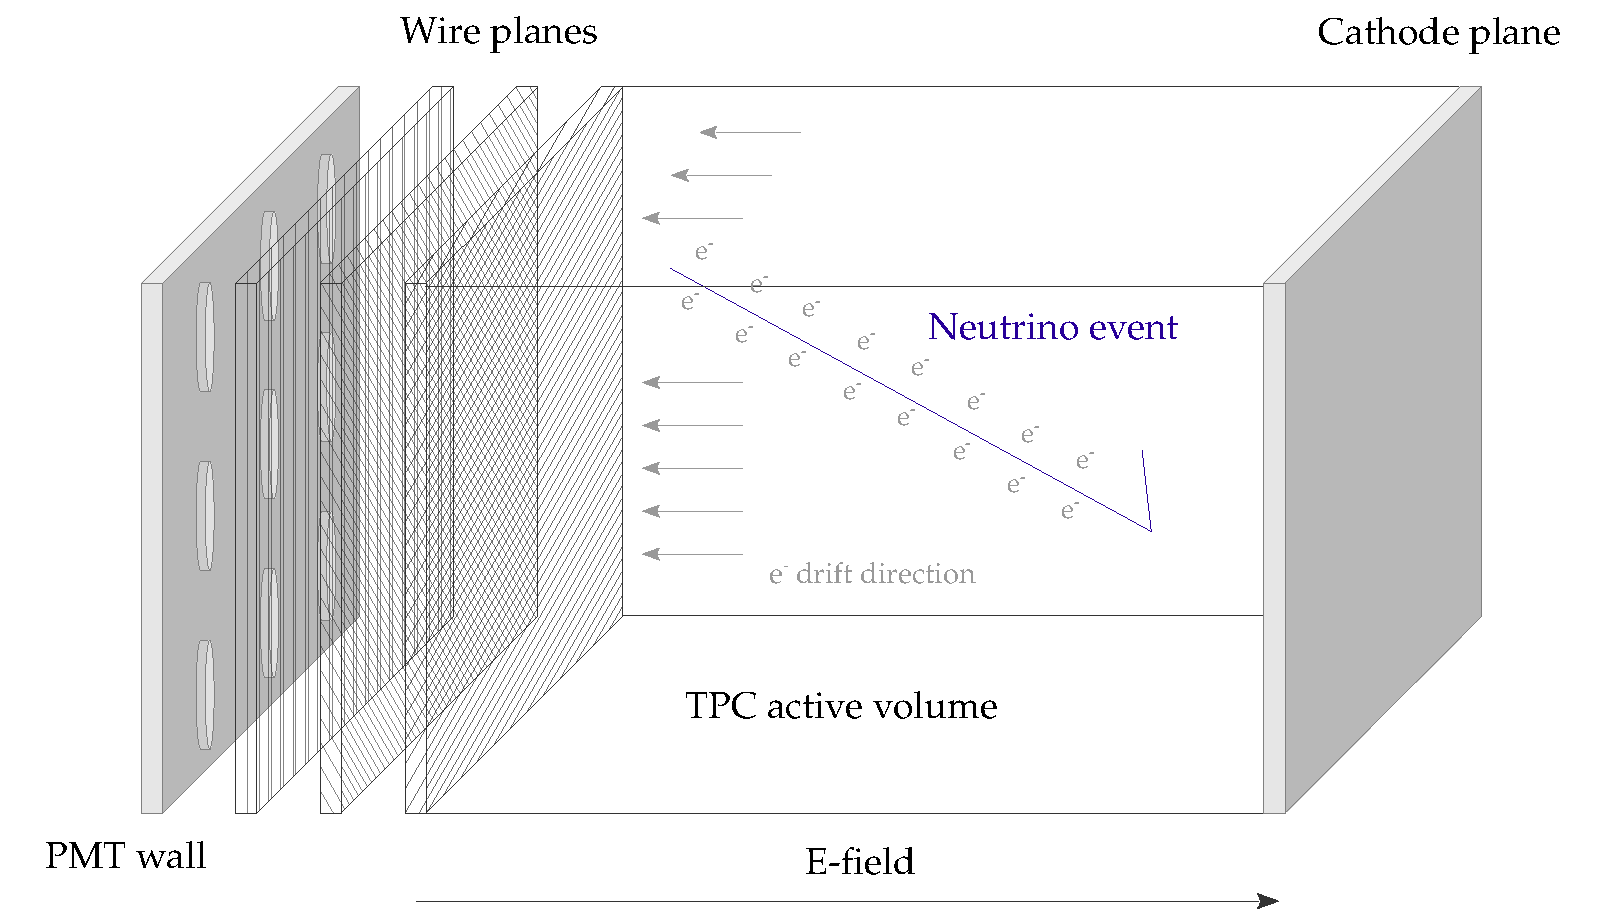
\includegraphics[width=.85\textwidth]{images/LArTPC.pdf}
        \caption{An example neutrino interaction within a typical LArTPC. The ionization electrons drift in what is defined as the positive x-direction as shown, and the scintillation light would be collected by the wall of PMTs behind the wire places. The induction planes U and V are at 60$^{\circ}$ to the vertical collection plane Y. The neutrino would enter the TPC in the positive z-direction.}
        \label{fig:lartpc}
    \end{figure}

\subsection{SBND}    

SBND will have a beamline of 110m, the shortest in the SBN program. At this distance, the flux of the neutrino beam is $\sim$100 times that of the other 2 SBN detectors, these relative fluxes are simulated as a function of neutrino energy and shown graphically in Figure~\ref{fig:sbnFlux} \cite{sbn}. Consequently, the number of events expected during the full exposure of the experiment is around 7,000,000. A breakdown in terms of individual processes is given in Figure~\ref{fig:sbndStats} \cite{sbn}. Combining these huge statistics with the exceptional resolution capabilities of the liquid argon TPCs will allow SBND to make unprecedentedly high-precision cross-section and oscillation measurements. Working both in conjuction with MicroBooNE and ICARUS, and as a stand-alone experiment, SBND should produce some exciting and extremely important results.

    % SBN fluxes
    \begin{figure}[h!]
        \center
        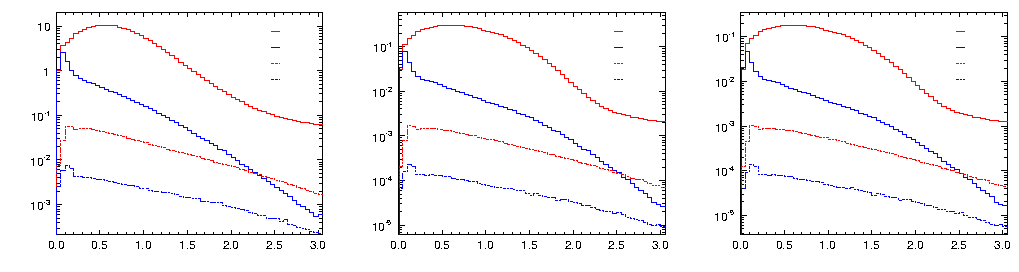
\includegraphics[width=\textwidth]{images/SBN_fluxes.pdf}
        \put(-45, -1){\scriptsize E$_{\nu}$ ( GeV )}
        \put(-192, -1){\scriptsize E$_{\nu}$ ( GeV )}
        \put(-340, -1){\scriptsize E$_{\nu}$ ( GeV )}
        \put(-438, 12){ \rotatebox{90}{\tiny $ \Phi ( \nu )_{ \mbox{SBND} } $/50 MeV /m$^{2}$/10$^{6}$ POT } }
        \put(-291, 12){ \rotatebox{90}{\tiny $ \Phi ( \nu )_{ \mu \mbox{BooNE} } $/50 MeV /m$^{2}$/10$^{6}$ POT } }
        \put(-144, 12){ \rotatebox{90}{\tiny $ \Phi ( \nu )_{ \mbox{ICARUS} } $/50 MeV /m$^{2}$/10$^{6}$ POT } }
        \put(-315, 102){\tiny $\nu_{\mu}$}
        \put(-315, 95){\tiny $\bar{\nu}_{\mu}$ }
        \put(-315, 88){\tiny $\nu_{e}$}
        \put(-315, 81){\tiny $\bar{\nu}_{e}$}
        \put(-168, 102){\tiny $\nu_{\mu}$}
        \put(-168, 95){\tiny $\bar{\nu}_{\mu}$ }
        \put(-168, 88){\tiny $\nu_{e}$}
        \put(-168, 81){\tiny $\bar{\nu}_{e}$}
        \put(-21, 102){\tiny $\nu_{\mu}$}
        \put(-21, 95){\tiny $\bar{\nu}_{\mu}$ }
        \put(-21, 88){\tiny $\nu_{e}$}
        \put(-21, 81){\tiny $\bar{\nu}_{e}$}
        \caption{From left to right, the BNB fluxes of SBND, MicroBooNE ($\mu$BooNE and ICARUS. From these plots it can be seen that SBND's flux will be $\sim$100 times the other two \cite{sbn}.}
        \label{fig:sbnFlux}
    \end{figure}
    
    % Table
    \begin{figure}[h!]
        \center
        \renewcommand{\arraystretch}{1.3}
\begin{center}
\begin{tabular}{lll}
    \textbf{Process} & & \textbf{No. Events} \\ 
    \hline\hline
    \multicolumn{3}{c}{\textit{\( \nu_{ \mu } \) Events }}\\
        CC 0 \( \pi \)                 & \( \nu_{ \mu } N \rightarrow \mu + Np \)                            & \textbf{3,551,830} \\
        CC 1 \( \pi^{ \pm } \)         & \( \nu_{ \mu } N \rightarrow \mu + nucleons +  1\pi^{ \pm } \)      & \textbf{1,161,610} \\
        CC \( \geq 2\pi^{ \pm } \)     & \( \nu_{ \mu } N \rightarrow \mu + nucleons + \geq 2\pi^{ \pm } \)  & 97,929 \\
        CC \( \geq 1\pi^{ 0 } \)       & \( \nu_{ \mu } N \rightarrow \mu + nucleons + \geq 1\pi^{ 0 } \)    & 497,963 \\
        \hline        
        NC 0 \( \pi \)                 & \( \nu_{ \mu } N \rightarrow nucleons \)                            & 1,371,070 \\
        NC 1 \( \pi^{ \pm } \)         & \( \nu_{ \mu } N \rightarrow nucleons +  1\pi^{ \pm } \)            & 260,924 \\
        NC \( \geq 2\pi^{ \pm } \)     & \( \nu_{ \mu } N \rightarrow nucleons + \geq 2\pi^{ \pm } \)        & 31,940 \\
        NC \( \geq 1\pi^{ 0 } \)       & \( \nu_{ \mu } N \rightarrow nucleons + \geq 1\pi^{ 0 } \)          & 358,443 \\
        \hline\hline
        \multicolumn{2}{l} {Total \( \nu_{ \mu } \) \& \( \nu_{ e } \) events }                              & \textbf{7,251,948} \\
\end{tabular}
\end{center}

        \caption{Some expected statistics for the entire exposure of SBND, broken down into some of the processes by which the neutrino may interact \cite{sbn}.}
        \label{fig:sbndStats}
    \end{figure}
    
    SBND will be 5m long, 4m tall and 4m wide holding a total of 112 tonnes of liquid argon in its active volume. As an LArTPC, SBND will function in mostly the same way as described earlier and in Figure~\ref{fig:lartpc}, although it will have some unique features. Figure~\ref{fig:sbndtpc} gives an idea of how the detector will be constructed. 
    
    % SBND TPC
    \begin{figure}[h!]
        \center
        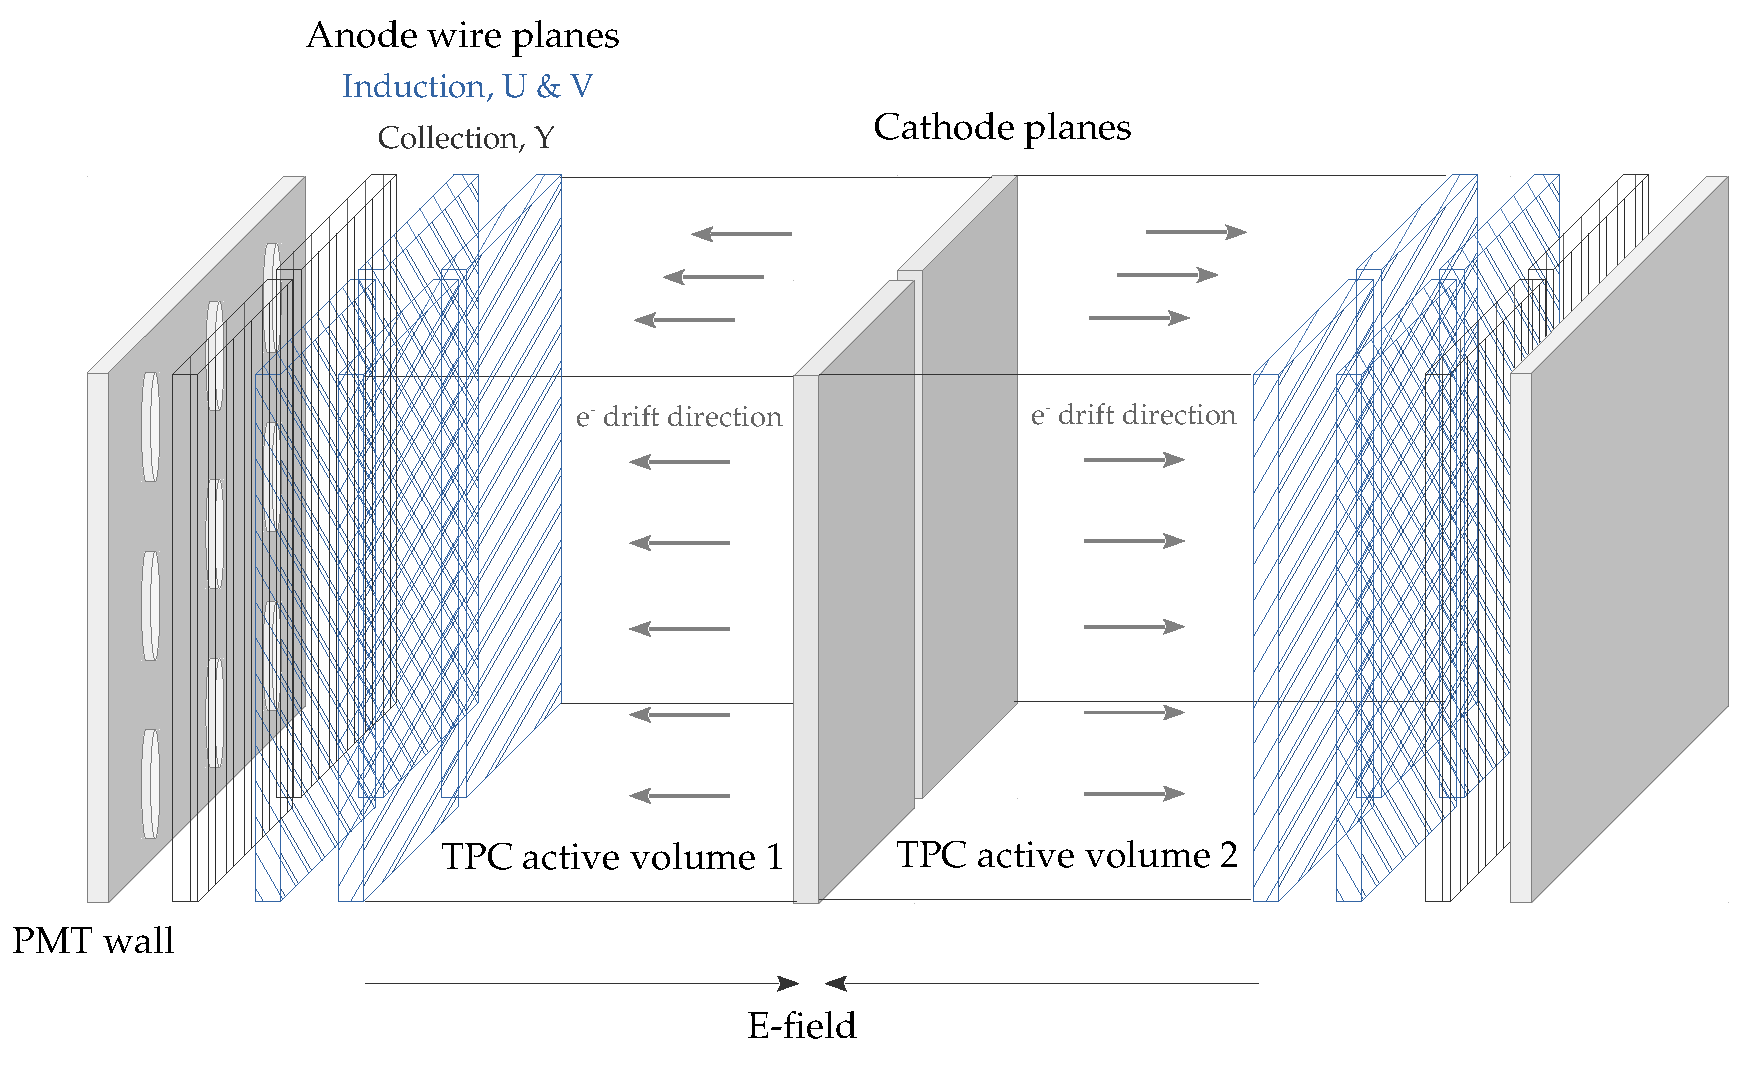
\includegraphics[width=.85\textwidth]{images/SBND_TPC.pdf}
        \caption{A diagram to give an idea of how the SBND detector will look. It features many similarities to the standard liquid argon TPC design, but applies the concept of multiple modules - this is a possibility for the structure of DUNE \cite{sbn}.}
        \label{fig:sbndtpc}
    \end{figure}
   
    \newpage 

    Unlike the typical TPC setup, SBND will have 2 cathode planes, 4 anode planes and 2 time projection chambers. The cathode planes will lie side-by-side, positioned at the join between the two TPCs. The anode planes will also lie in twos next to one another, with a pair residing on the opposite wall to the cathode plane of each TPC. This allows for 2 electric fields and therefore 2 opposing drift directions. In the same way as shown in Figure~\ref{fig:lartpc}, there will be 3 wire planes to each anode plane. In the gaps between two adjacent anode planes, electrodes will divert the approaching particles towards the nearest active parts of the plane \cite{sbn}. The multiple module system may well be a feature of the next generation TPC detectors such as DUNE. 

\clearpage
